
\documentclass[10pt]{beamer}
\hypersetup{
        unicode=true,
        linkcolor=blue,
        anchorcolor=blue,
        citecolor=green,
        filecolor=black,
        urlcolor=blue
    }

% https://github.com/uta-smile/beamer-theme/blob/master/example.tex


% Font
%\usefonttheme{professionalfonts}
%\usepackage{arev}
\usepackage{newtxsf}

%%%%% PACKAGES HERE
%% \usepackage{}
\usepackage{amsmath}
\usepackage{amssymb}
\usepackage{listings}
\usepackage[cache=false]{minted}
\usepackage{textcomp}

% Eingabecodierung
\usepackage[utf8]{inputenc}

% Sprachraum
\usepackage[ngerman]{babel}

% Bilder einbinden
\usepackage{graphicx}
\graphicspath{{images/}}

% Zeichnen
\usepackage{tikz}
\usepackage{mathtools}
\usepackage{amsmath,amsfonts,amssymb}
\usepackage{tikz}
\usetikzlibrary{automata,positioning}
\usepackage{amsmath,verbatimbox}

% Grafiken zeichen
\usepackage{tikz}
\usetikzlibrary{calc,arrows,positioning} 
\usepackage{pgfplots}
\pgfplotsset{compat=1.7}
\def\checkmark{\tikz\fill[scale=0.4](0,.35) -- (.25,0) -- (1,.7) -- (.25,.15) -- cycle;} 

% Pie Chart
% https://tex.stackexchange.com/questions/500362/using-pgf-pie-to-draw-pie-charts-without-labels-on-the-slices-but-still-able-to
\usepackage{pgf-pie}
\usepackage{etoolbox}
\newtoggle{showpct}
\makeatletter
\patchcmd{\pgfpie@slice}%
{\pgfpie@scalefont{#3}\pgfpie@numbertext{#3}}%
{\iftoggle{showpct}{\pgfpie@scalefont{#3}\pgfpie@numbertext{#3}}{}}%
{}{}
\makeatother

% Code
\usepackage{listings}

% https://tex.stackexchange.com/questions/16979/columns-with-latex-code-and-output-in-a-beamer-presentation
\usepackage{showexpl} 
\lstloadlanguages{[LaTeX]Tex} 
\lstset{% 
     basicstyle=\ttfamily\small, 
     commentstyle=\itshape\ttfamily\small, 
     showspaces=false, 
     showstringspaces=false, 
     breaklines=true, 
     breakautoindent=true, 
     captionpos=t 
} 

\usepackage[babel, german=quotes]{csquotes}
\usepackage[
backend=biber,
style=numeric-comp,
block=ragged,			
sorting=none,			
]{biblatex}
\addbibresource{references.bib}

%%%%%%%%%%%%%%%%%%%%%%%%%%%%%%%%%%%
%% DO NOT CHANGE

\usetheme{default}
\useinnertheme{circles}
\useoutertheme{infolines}
\usefonttheme{serif}

\usepackage{etoolbox}

%% T for navigation symbols
%%\setbeamertemplate{navigation symbols}{}

%% T for header
%% \setbeamertemplate{headline}{%
%%   \leavevmode%
%%   \ifdefempty{\insertsubsectionhead}{
%%     \begin{beamercolorbox}[wd=0.99\paperwidth,ht=2.25ex,dp=1ex,center]{section in head/foot}%
%%       % \hbox to .5\paperwidth{\hfil\insertsectionhead\hfil}
%%       \insertsectionhead
%%     \end{beamercolorbox}%
%%   }{
%%     \begin{beamercolorbox}[wd=.44\paperwidth,ht=2.25ex,dp=1ex,right]{section in head/foot}%
%%       % \hbox to .5\paperwidth{\hfil\insertsectionhead\hfil}
%%       \insertsectionhead
%%     \end{beamercolorbox}%
%%     \begin{beamercolorbox}[wd=.1\paperwidth,ht=2.25ex,dp=1ex,center]{section in head/foot}%
%%       % \hbox to .5\paperwidth{\hfil\insertsectionhead\hfil}
%%       -
%%     \end{beamercolorbox}%
%%     \begin{beamercolorbox}[wd=.44\paperwidth,ht=2.25ex,dp=1ex,left]{subsection in head/foot}%
%%       % \hbox to .5\paperwidth{\hfil\insertsubsectionhead\hfil}
%%       \insertsubsectionhead
%%     \end{beamercolorbox}
%%   }%
%% }

%% T for frame title
\setbeamertemplate{frametitle}{%
  \usebeamerfont{frametitle}\insertframetitle\strut%
  \vskip-0\baselineskip%
  \leaders\vrule width .95\paperwidth\vskip1pt%
  \vskip0pt%
  \nointerlineskip
}

%% T for footer
\setbeamercolor{footlinecolor}{fg=cyan,bg=green}
\setbeamercolor{author in head/foot}{fg=blue}

\setbeamercolor{alerted text}{fg=orange}

\setbeamertemplate{footline}{%
  \leavevmode%
  \hbox{%
  \begin{beamercolorbox}[wd=.4\paperwidth,ht=2.25ex,dp=1ex,left]{author in head/foot}%
    \hspace*{2ex}\usebeamerfont{author in head/foot} Löst das Chainweb das Blockchaintrilemma?
  \end{beamercolorbox}%

  \begin{beamercolorbox}[wd=.6\paperwidth,ht=2.25ex,dp=1ex,right]{date in head/foot}%
    \usebeamerfont{date in head/foot}
    \insertshortdate{}\hspace*{1em}  % date
    \insertframenumber/\inserttotalframenumber\hspace*{2ex}
  \end{beamercolorbox}}%
  \vskip0pt%
}
%%%%%%%%%%%%%%%%%%%%%%%%%%%%%%%%%%%%%%%%%%%%%%%%

%% Start from here.
\title{Löst das Chainweb das Blockchaintrilemma?}
\author{Name}
\date\today

\begin{document}

\begin{frame}[plain]
	\titlepage
\end{frame}


\begin{frame}{Inhaltsverzeichnis}
	\tableofcontents
\end{frame}

\section{Grundlagen der Blockchaintechnologie}

\subsection {Grundlagen}
\begin{frame}
	\frametitle{Grundlagen}
	\begin{itemize}
		\item Hashfunktion: $h : \{0,1\}^* \rightarrow \{0,1\}^l$
		      \begin{itemize}
		      	\item $h$ für Computer einfach zu berechnen
		      	\item Es gilt für alle $x$ und ${x}'$: $h(x) \neq h({x}')$
		      \end{itemize}
		\item Bestätigung von Transaktionen durch Rechenleistung: Proof of Work
		\item Limitierter Durchfluss (TPS) von etwa 5 Transaktionen pro Sekunde
	\end{itemize}
\end{frame}

\subsection {Proof of Work}
\begin{frame}{Proof of Work}
	\begin{itemize}
		\item Berechnen des Hashwertes mit verschiendenen Werten für die Nonce
	\end{itemize}
	
	\begin{figure}
		\centering
		\begin{minipage}{0.33\textwidth}
			\centering
			\begin{tikzpicture}
				\draw (0,0) rectangle (2,3) node[align=center, pos=.5] {
					$A \xrightarrow{\text{5}} B$\\
					$A \xrightarrow{\text{9}} C$\\ 
					<...>\\\\
					Nonce \\
					64392
				};
				\draw (0,1) rectangle (2,1);
				\draw (0,0) -- (1,-1) -- (2,0);    
				\node[draw] at (1,-1.5) {\textcolor{red}{3836253623673124}};
			\end{tikzpicture}
		\end{minipage}\hfill
		\begin{minipage}{0.33\textwidth}
			\centering
			\begin{tikzpicture}
				\draw (0,0) rectangle (2,3) node[align=center, pos=.5] {
					$A \xrightarrow{\text{5}} B$\\
					$A \xrightarrow{\text{9}} C$\\ 
					<...>\\\\
					Nonce \\
					09203
				};
				\draw (0,1) rectangle (2,1);
				\draw (0,0) -- (1,-1) -- (2,0);    
				\node[draw] at (1,-1.5) {\textcolor{red}{0303948571920435}};
			\end{tikzpicture}
		\end{minipage}
		\begin{minipage}{0.33\textwidth}
			\centering
			\begin{tikzpicture}
				\draw (0,0) rectangle (2,3) node[align=center, pos=.5] {
					$A \xrightarrow{\text{5}} B$\\
					$A \xrightarrow{\text{9}} C$\\ 
					<...>\\\\
					Nonce \\
					94832
				};
				\draw (0,1) rectangle (2,1);
				\draw (0,0) -- (1,-1) -- (2,0);    
				\node[draw] at (1,-1.5) {\textcolor{green}{\textbf{00000000}23673124}};
			\end{tikzpicture}
		\end{minipage}
	\end{figure}
\end{frame}


\begin{frame}{Proof of Work}
	\begin{itemize}
		\item Einreihen gefundener Blöcke in die Blockchain
	\end{itemize}
	\begin{figure}[h!]
		\centering
		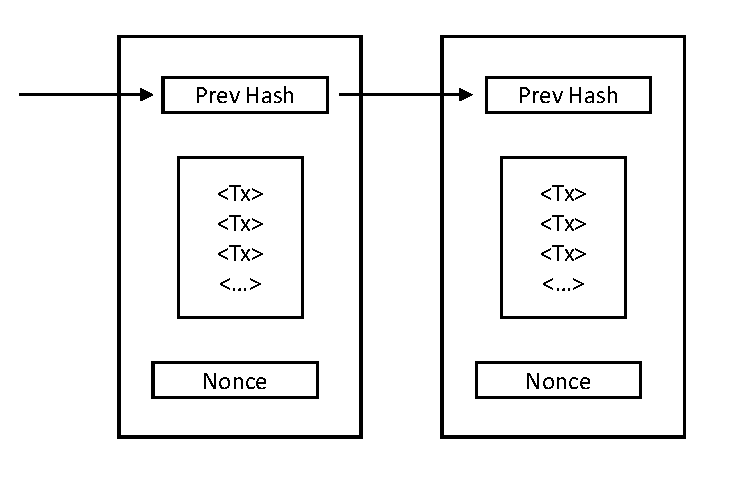
\includegraphics[width=0.5\linewidth]{blockchain_nonce_pdf_cropped.pdf}
		\caption{Vereinfachte Darstellung einer Blockchain. \cite{Nakamoto.2009}} 
	\end{figure}
\end{frame}


\subsection {Blockchaintrilemma}
\begin{frame}{Blockchaintrilemma}
	Vereinen dreier wünschenswerter Faktoren einer Blockchain:
	\begin{itemize}
		\item Dezentral
		\item Skalierbarkeit
		\item Sicher
	\end{itemize}
\end{frame}


\section {Chainweb}
\subsection {Überblick}
\begin{frame}
	\frametitle{Funktionsweise des Chainwebs}
	\begin{itemize}
		\item Proof of Work
		\item Mehrere parallele, unabhängige Ketten
		\item Jede Kette referenziert neben Vorgängerblock auch auf andere Ketten
	\end{itemize}
	    
	    
	\begin{figure}[h!]
		\usetikzlibrary{graphs,graphs.standard}
		\tikzgraphsset{edges={draw,semithick}, nodes={circle,draw,semithick}}
		\centering
		\tikz \graph[math nodes, clockwise]
		{ subgraph I_n [V={0,1,2,3,4}] --
			subgraph C_n [V={5,6,7,8,9},
			radius=1.25cm];
			{[cycle] 0,2,4,1,3} };
		\caption{Petersen-Graph der Ordnung 10, Grad 3 und Durchmesser 2. \cite{Martino.2018}} 
		\label{fig:petersen_graph_10}
	\end{figure}
\end{frame}

\subsection{Durchfluss}
\begin{frame}{Durchfluss des Chainwebs}
	\begin{itemize}
		\item Durchfluss von einer Kette $TPS_1 = 8$ experimentell bestimmt
		\item Gesammtdurchfluss mit $C$ Ketten: $TPS_C = C \cdot 8$
		              
	\end{itemize}
	\begin{figure}[h!]
		\begin{tikzpicture}[thick,scale=0.8, every node/.style={scale=0.8}]
			\begin{axis}[ 
					xlabel=$Ketten \ C$,
					ylabel={$TPS$}
				] 
				\addplot[domain=0:5000] {x*8}; 
			\end{axis}
		\end{tikzpicture}
		\caption{Darstellung des Durchflusses in Abhängigkeit der Ketten.}
		\label{fig:tps_chain}
	\end{figure}
\end{frame}

\subsection{Zusammenfassung}
\begin{frame}{Zusammenfassung}
	\begin{itemize}
		\item Skalierbar \checkmark
		\item Theoretisch dezentral \checkmark
		\item Sicher \checkmark
		              
	\end{itemize}
\end{frame}

\section{Umsetzung in \LaTeX}
\subsection{Codebeispiele}
\begin{frame}[fragile]{Petersen-Graph}
	\begin{columns}
		\begin{column}{0.5\textwidth}
			\begin{lstlisting}
\usetikzlibrary{
  graphs,graphs.standard
}
\tikzgraphsset{
  edges={draw,semithick}, 
  nodes={circle,draw,semithick}
}
\centering
\tikz 
\graph[math nodes, clockwise]
{ subgraph I_n [V={0,1,2,3,4}] --
  subgraph C_n [V={5,6,7,8,9},
  radius=1.25cm];
{[cycle] 0,2,4,1,3} };
    \end{lstlisting}
		\end{column}
		\begin{column}{0.5\textwidth}  
			\begin{center}
				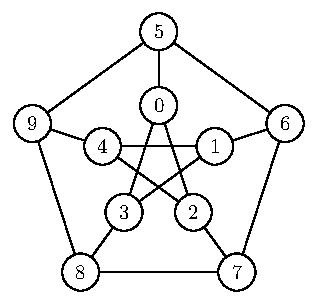
\includegraphics[width=\textwidth]{graph.pdf}
			\end{center}
		\end{column}
	\end{columns}
\end{frame}

\begin{frame}{Kreisdiagramm}
	\begin{figure}[h]
		\centering
		\togglefalse{showpct}
		\begin{tikzpicture}
			\tikzset{lines/.style={draw=white},}
			\pie[color = {cyan, red, blue!80, yellow, green, purple!80},
				sum=auto, 
				after number=,
				text=legend,
			style={lines}]
			{68.03/A,17.36/B,5.01/C,2.34/D,2.11/E,5.14/F}
		\end{tikzpicture}
		\caption{Kreisdiagramm in \LaTeX.}
		\label{fig:chainweb_miner}
	\end{figure}
\end{frame}

\begin{frame}[fragile]{Kreisdiagram}
	\begin{itemize}
		\item Modifizieren des Pakets $pgf-pie$ durch $etoolbox$
	\end{itemize}
	\begin{lstlisting}
        % Präambel
        \usepackage{pgf-pie}
        \usepackage{etoolbox}
        \newtoggle{showpct}
        \makeatletter
        \patchcmd{\pgfpie@slice}%
        {\pgfpie@scalefont{#3}\pgfpie@numbertext{#3}}%
        {\iftoggle{showpct}{\pgfpie@scalefont{#3}
        \pgfpie@numbertext{#3}}{}}%
        {}{}
        \makeatother
        \end{lstlisting}
\end{frame}

\section{Schlussbemerkung}
\begin{frame}{Schlussbemerkung}
	\begin{itemize}[<+- | alert@+>]
		\item Zu jedem Problem gab es irgendwo eine passende Lösung
		\item Effiziente Nummerierung von Bildern, Formeln und Abschnitten
		\item \LaTeX \ hat mich überzeugt
	\end{itemize}
\end{frame}

\section{}
\begin{frame}
  % frame contents here
\end{frame}


\nocite{*}
\begin{frame}[allowframebreaks]{Literatur}
    \printbibliography[]
\end{frame}
\end{document}